\begin{figure}
\centering
\hspace*{-0.1cm}
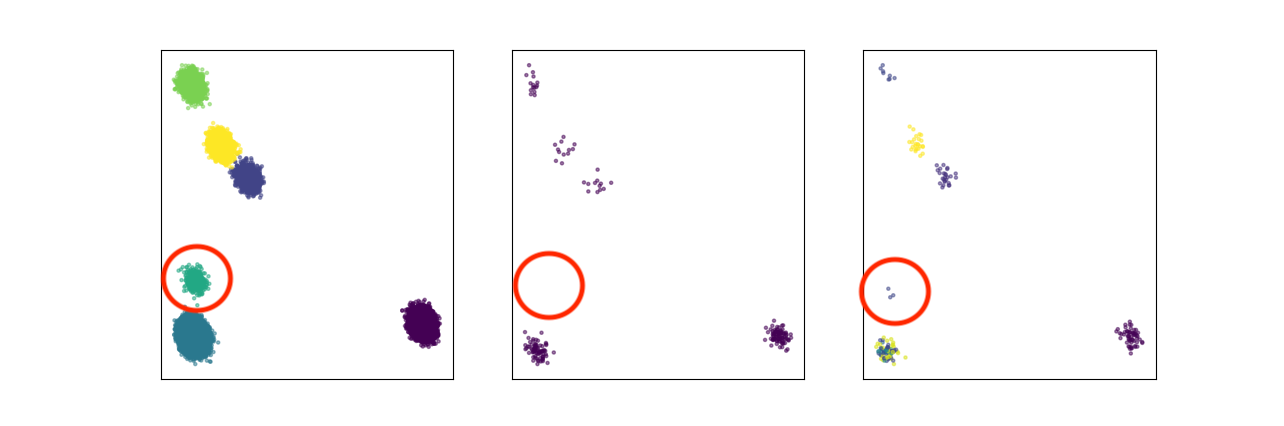
\includegraphics[trim={4cm 0 0 0},clip,width=1.13\linewidth]{images/lightweight_breaks.png}
\vspace*{-0.8cm}
\caption{
The results of lightweight and fast-coreset constructions on a 2D Gaussian mixture dataset of $n=100K$ points with clusters of varying size. The circled cluster has $\sim 400$
points and coresets have 200 points.
\emph{Left}: Original multivariate-Gaussian dataset.
\emph{Middle}: Lightweight coresets fail to capture the cluster of $\sim$ 400 points.
\emph{Right}: Sensitivity sampling with $j=k$ identifies all of the clusters.
}
\label{fig:lightweight_breaks}
\end{figure}
